對於有$V$個點、$E$條邊、$F$個面(含外部)的連通平面圖
\normalsize \[ F+V-E=2 \]
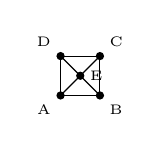
\begin{tikzpicture}         % Graph 1
    % 定義頂點的位置
    \coordinate (A) at (0, 0);
    \coordinate (B) at (0.5, 0);
    \coordinate (C) at (0.5, 0.5);
    \coordinate (D) at (0, 0.5);
    \coordinate (E) at (0.25, 0.25);
    
    % 畫出頂點
    \fill (A) circle (1.5pt) node[below left, font=\tiny] {A};
    \fill (B) circle (1.5pt) node[below right, font=\tiny] {B};
    \fill (C) circle (1.5pt) node[above right, font=\tiny] {C};
    \fill (D) circle (1.5pt) node[above left, font=\tiny] {D};
    \fill (E) circle (1.5pt) node[right, font=\tiny] {E};
    
    % 畫出邊
    \draw (A) -- (B);
    \draw (A) -- (D);
    \draw (A) -- (E);
    \draw (B) -- (C);
    \draw (B) -- (E);
    \draw (C) -- (D);
    \draw (C) -- (E);
    \draw (D) -- (E);
\end{tikzpicture}
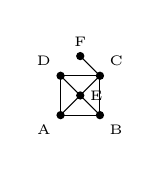
\begin{tikzpicture}         % Graph 2
    % 定義頂點的位置
    \coordinate (A) at (0, 0);
    \coordinate (B) at (0.5, 0);
    \coordinate (C) at (0.5, 0.5);
    \coordinate (D) at (0, 0.5);
    \coordinate (E) at (0.25, 0.25);
    \coordinate (F) at (0.25, 0.75);
    
    % 畫出頂點
    \fill (A) circle (1.5pt) node[below left, font=\tiny] {A};
    \fill (B) circle (1.5pt) node[below right, font=\tiny] {B};
    \fill (C) circle (1.5pt) node[above right, font=\tiny] {C};
    \fill (D) circle (1.5pt) node[above left, font=\tiny] {D};
    \fill (E) circle (1.5pt) node[right, font=\tiny] {E};
    \fill (F) circle (1.5pt) node[above, font=\tiny] {F};
    
    % 畫出邊
    \draw (A) -- (B);
    \draw (A) -- (D);
    \draw (A) -- (E);
    \draw (B) -- (C);
    \draw (B) -- (E);
    \draw (C) -- (D);
    \draw (C) -- (E);
    \draw (C) -- (F);
    \draw (D) -- (E);
\end{tikzpicture}
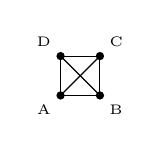
\begin{tikzpicture}         % Graph 3
    % 定義頂點的位置
    \coordinate (A) at (0, 0);
    \coordinate (B) at (0.5, 0);
    \coordinate (C) at (0.5, 0.5);
    \coordinate (D) at (0, 0.5);
    
    % 畫出頂點
    \fill (A) circle (1.5pt) node[below left, font=\tiny] {A};
    \fill (B) circle (1.5pt) node[below right, font=\tiny] {B};
    \fill (C) circle (1.5pt) node[above right, font=\tiny] {C};
    \fill (D) circle (1.5pt) node[above left, font=\tiny] {D};
    
    % 畫出邊
    \draw (A) -- (B);
    \draw (A) -- (C);
    \draw (A) -- (D);
    \draw (B) -- (C);
    \draw (B) -- (D);
    \draw (C) -- (D);
\end{tikzpicture}
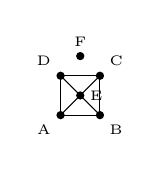
\begin{tikzpicture}         % Graph 4
    % 定義頂點的位置
    \coordinate (A) at (0, 0);
    \coordinate (B) at (0.5, 0);
    \coordinate (C) at (0.5, 0.5);
    \coordinate (D) at (0, 0.5);
    \coordinate (E) at (0.25, 0.25);
    \coordinate (F) at (0.25, 0.75);
    
    % 畫出頂點
    \fill (A) circle (1.5pt) node[below left, font=\tiny] {A};
    \fill (B) circle (1.5pt) node[below right, font=\tiny] {B};
    \fill (C) circle (1.5pt) node[above right, font=\tiny] {C};
    \fill (D) circle (1.5pt) node[above left, font=\tiny] {D};
    \fill (E) circle (1.5pt) node[right, font=\tiny] {E};
    \fill (F) circle (1.5pt) node[above, font=\tiny] {F};
    
    % 畫出邊
    \draw (A) -- (B);
    \draw (A) -- (D);
    \draw (A) -- (E);
    \draw (B) -- (C);
    \draw (B) -- (E);
    \draw (C) -- (D);
    \draw (C) -- (E);
    \draw (D) -- (E);
\end{tikzpicture}
\begin{tiny}
    (1)、(2)正確;(3)$\overline{AC}$與$\overline{BD}$相交,錯誤;(4)非連通圖
\end{tiny}